\section{Prototype 2}
\label{ap:prototype2}

Afprøvning af Prototype 2 på Merete er blevet filmet\cite{prototype2merete}.

Afprøvning af Prototype 2 på Keld er blevet filmet\cite{prototype2keld}.

\begin{description}
\item[Formål] På baggrund af møde 2, hvor informanterne kom med krav til systemets funktioner, har vi nu lavet en diasshow-prototype på gomockingbird.com, hvor systemets funktion er vist. Når informanterne præsenteres for funktionerne i noget der, med lidt god vilje, ligner en rigtig hjemmeside, så kan det være at informanten bliver klar over at en funktion enten mangler, eller at en tidligere foreslået funktion er overflødig. Formålet med mødet er derfor primært at ud af, om der er de funktioner, som informanten har brug for. Derudover vil vi også gerne finde ud af om brugeren kan finde de nødvendige funktioner, altså om programmet og dets funktioner som helhed er intuitive at bruge for informanterne.
\begin{figure}[H]
\centering
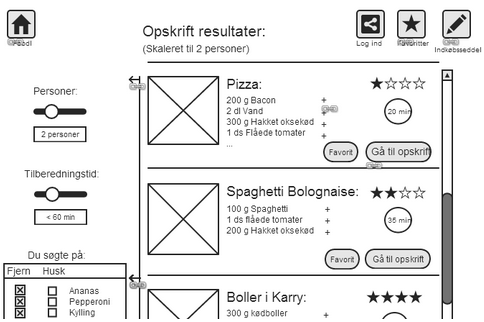
\includegraphics[scale=0.7]{billeder/prototyper/prototype2.png}
\capt{Visualisering af prototype 2.}
\label{fig:prototype2}
\end{figure}

Først udføres en case for at få ledt brugeren rundt blandt alle funktionerne.

\item[Case] Følgende case blev udført af informanterne.

\begin{enumerate}[noitemsep]
\item Udfør en søgning på ingredienserne (pepperoni, ananas og kylling). Ingredienser tilføjes ved at klikke i søgefeltet
\item Skjul alle opskrifter med nødder
\item Gå til den første opskrift, der fremkommer
\item Gå tilbage og tilføj 200 g Bacon (fra pizzaens ingredienser) til din indkøbsliste
\item Print indkøbslisten ud
\item Gør klar til en helt ny søgning
\item Foretag en søgning på pepperoni
\item Du fandt ingen opskrifter, så du vil gerne tilføj ananas, inden du søger igen (du søger altså på pepperoni og ananas)
\item Føj den første opskrift, du finder, til dine favoritter
\end{enumerate}

Efter casen tages en snak om hver af disse funktioner og muligheder med systemet.

Informanten bliver præsenteret for mange funktioner, hvor vi her beskriver hvad deres mening var omkring disse funktioner efter at have udført casen.

\begin{itemize}[noitemsep]
\item Begrænse søgeresultat efter tilberedningstid
\begin{itemize}[noitemsep]
\item Merete synes idéen er god, men foreslår nu kun 2 valgmuligheder ``kort'' eller ``lang'' tilberedningstid
\item Keld synes også dette er en god ide. En opdeling på en 30 min. burde være fint, måske 15 min. Hvis det er tilberedningstid på over en time, må skalaen godt springe mere end 15-30 min.
\end{itemize}
\item Sidebar
\begin{itemize}[noitemsep]
\item Merete opdagede ikke at denne sidebar kunne trækkes ud
\item Den ligger ikke logisk for en. Selvom den er stor. Den bliver skjult i designet
\item Keld synes ikke det ser for rodet ud, selvom sidebaren er ude hele tiden
\end{itemize}
\item Skalere en opskrift til x personer
\begin{itemize}[noitemsep]
\item Merete ser det som en nyttig funktion, hun vil skalere til mellem 2-4 personer
\item Det er en god funktion, som Keld er sikker på mange vil få brug for. Opskalering til 5 burde være nok. Måske 1-20, så er gæstebehov også dækket ind. Men det er trods alt til rester, så til 5 personer burde være nok.
\end{itemize}
\item Fjerne ingredienser inden en søgning udføres (på forsiden)
\begin{itemize}[noitemsep]
\item Merete synes det er meget brugbart
\item Keld synes det er fint at det er på forsiden
\end{itemize}
\item Fjerne ingredienser efter en søgning er udført (på søgeresultatsiden)
\begin{itemize}[noitemsep]
\item Merete synes idéen med at kunne fjerne ingredienser mens der vises søgeresultater er god
\item Keld synes det er fint, at det også er muligt i sidebaren
\end{itemize}
\item Huske ingredienser til næste søgning
\begin{itemize}[noitemsep]
\item Merete synes måden det fungerer på i prototypen er god. Hun vil ikke have at de huskede ingredienser vises på forsiden
\item Keld synes det er rart at det er muligt at huske nogle ingredienser. Det ville måske også være rart, hvis det også var muligt at gøre fra forsiden. Keld er dog i tvivl om, hvor på forsiden det skulle være. Det er måske alligevel bedst hvis forsiden er simpel. Han synes funktionen er brugbar
\end{itemize}
\item Skjule opskrifter indeholdende bestemte ting
\begin{itemize}[noitemsep]
\item Merete synes det virker godt
\item Keld synes det er en god ide. Han fik hurtigt fundet funktionen, så snart toolboxen blev åbnet
\end{itemize}
\item Browsers tilbageknap går til forsiden (beholder ingredienser)
\begin{itemize}[noitemsep]
\item Merete opdagede ikke denne funktion
\item Keld opdagede funktionen, og anvendte den også. Måske ville en tilbage- og fremknap på selve siden være brugbar, foreslår Keld
\end{itemize}
\item Home knap går tilbage (fjerne ingredienser)
\begin{itemize}[noitemsep]
\item Merete synes det virkede naturligt
\item Keld synes det er godt at have en kanp som går helt tilbage. Men han foreslår endnu engang at have en frem- og tilbageknap som supplerer home-knappen
\end{itemize}
\item Visning af opskrifter (ekspander ved mouse over)
\begin{itemize}[noitemsep]
\item Merete synes opskrifterne blev vist fint. Hun kunne godt lide idéen med at ekspandere opskriften ved mouseover
\item Keld synes bare man skal have vist de væsentligste ingredienser. Han synes det ville være smart, hvis det var muligt at se hele ingredienslisten ved hjælp af et mouse-over
\end{itemize}
\item Gå til opskrifter (evt link ved klik på navn)
\begin{itemize}[noitemsep]
\item Merete synes ikke knappen “Gå til opskrift”, er overflødig. Hun ville blive forvirret hvis den ikke var der, og man bare skulle trykke et sted på opskriften (navnet, eller baggrunden, hvor baggrundsfarve ændrer sig eller lignende)
\item Keld synes det er godt med en “Gå til opskrift”-knap. Det er brugervenligt
\end{itemize}
\item Tilføj opskrift til favoritter
\begin{itemize}[noitemsep]
\item Merete synes ikke man skal gå fra et søgeresultat og over til favoritsiden hver gang man tilføjer en opskrift til favoritter. Opskriften skal blot tilføjes. Måske den skal sige en lyd og fjerne knappen man trykkede på. Favoritter-ikonet kunne lyse op
\item Skal lave en “Fjern fra favorit-knap”, så man hurtigt kan ombestemme sig
\item Keld synes det er smart nok at man sendes ind på favoritlisten, så man er sikker på at opskriften er kommet derind. Havde man samtidig en frem- og tilbageknap ville det være endnu bedre
\end{itemize}
\item Favoritter (knappen, der viser ens favoritter)
\begin{itemize}[noitemsep]
\item Merete var lidt forvirret med hensyn til om den tilføjede en opskrift til favoritter, eller hvad den gjorde
\item Keld synes at det skal være muligt at skalere opskrifterne på favoritsiden og at det er muligt nemt at fjerne opskrift fra favoritsiden igen
\end{itemize}
\item Visning af favoritter (layout)
\begin{itemize}[noitemsep]
\item Merete syntes layoutet var godt, og kunne godt lide at det mindede om layoutet ved visning af søgeresultat
\item Keld synes godt om layoutet
\end{itemize}
\item Visning af indkøbsliste
\begin{itemize}[noitemsep]
\item Merete synes det er en god idé at man kan tilføje tekst
\item Keld foreslår at man har ingredienslisten fra den opskrift man har været inde på, ved siden af indkøbslisten, så det er muligt hurtigt at tilføje flere ingredienser derfra
\item Keld synes indkøbslisten er meget brugbar. Det er for ofte man glemmer nogle ting, uden indkøbslisten
\end{itemize}
\item Tilføje opskrifts ingredienser til indkøbsliste
\begin{itemize}[noitemsep]
\item Merete vidste ikke hvordan man gjorde. Hun troede ikke man kunne trykke på +’et
\item Keld kunne godt tilføje en ingrediens til indkøbslisten
\end{itemize}
\item Home-knappen sender en til en helt tom forside
\begin{itemize}[noitemsep]
\item Merete kunne godt lide dette. Det virkede helt naturligt for hende
\item Keld synes det giver mening
\end{itemize}
\item Logge ind (få afklaret med brugeren, hvordan det skal foregå)
\begin{itemize}[noitemsep]
\item Log ind mest forståeligt
\item Kender meget til login, intet til synkronisering
\item Log ind er klart mest forståeligt for Keld. Keld har ikke lyst til at indtaste mere end mail-adresse, navn eller brugernavn og adgangskode. Helst ikke mere end det. Det er fint at der kommer en bekræftelsesmail til ens indbakke, men helst ikke aktiveringsmail
\item Sikkerheden har ikke høj-prioritet for Keld, da der alligevel ikke er nogle følsomme informationer på siden
\end{itemize}
\item Informants forslag til flere funktion
\begin{itemize}[noitemsep]
\item Merete havde ingen forslag, udover at der skal være billede af opskrifterne, hvilket ikke var vist i prototypen
\item Keld foreslår at sidebaren også er på favoritsiden
\item Keld foreslår en frem- og tilbageknap
\item Filtrering af forskellige landes køkkener, så det eksempelvis var muligt at se italienske retter, kinesiske retter osv. (kun de mest kendte køkkener: nordiskekøkken, kinesiske, italienske, græske \fx)
\end{itemize}
\end{itemize}
\end{description}

\subsection{Sammendrag}

I forhold til funktionalitet i prototype 2, er der nogle få ting, der skal tilføjes, fjernes eller ændres:

\begin{enumerate}[noitemsep]
\item Når man på søgesiden tilføjer en opskrift til favoritter, skal man forblive på søgesiden. Knappen man trykkede på skal erstattes med en ``Fjern fra favoritter''-knap
\item Sidebaren på søgeresultatssiden skal være nemmere at få øje på. En løsning er at gøre den synlig fra starten og give brugeren muligheden for at skjule den
\item Knappen i toppen, der viser de favoritter man har gemt, skal være mere sigende. ``Vis favoritter'' kunne der stå under den
\item På søgeresultatsiden, hvor en opskrifts vises, skal +’et ud for ingredienserne, der tilføjer en ingrediensen til indkøbslisten, være mere intuitiv
\item Brugeren skal muligvis have at vide, at man kan benytte browserens tilbageknap for at gå tilbage til forsiden, uden at ingredienser fjernes. Det kan være at informanten overså denne funktion fordi prototypen blev vist i form af et diasshow på en hjemmeside, og informanten derfor var bange for at gå væk fra hele diasshowets side
\item Skalering og andre funktioner til visning af favoritter
\item Frem og tilbage knap, der giver brugeren tryghed når han navigerer rundt, så man ikke skal være bange for at browseren forsvinder fra siden
\end{enumerate}
